\documentclass[12pt]{report}
\usepackage[a4paper,margin=1in]{geometry}
\usepackage{graphicx}
\usepackage{hyperref}
\usepackage{listings}
\usepackage{color}
\usepackage{tikz}
\usetikzlibrary{positioning,arrows.meta,shapes,fit}
\usepackage{pgfplots}
\pgfplotsset{compat=1.17}
\usepackage{longtable}
\usepackage{booktabs}
\usepackage{enumitem}
\usepackage{float}
\usepackage{caption}
\usepackage{subcaption}

\linespread{1.15}

\definecolor{codebg}{rgb}{0.96,0.96,0.96}
\definecolor{codefg}{rgb}{0.1,0.1,0.1}

\lstset{
  basicstyle=\small\ttfamily\color{codefg},
  backgroundcolor=\color{codebg},
  frame=single,
  breaklines=true,
  showstringspaces=false,
  tabsize=2,
  captionpos=b
}

\title{PolyStoreBench \\ Detailed report and beginner guide}
\author{}
\date{May 4, 2026}

\begin{document}
\maketitle
\tableofcontents
\listoffigures
\lstlistoflistings

\chapter{Introduction}
PolyStoreBench is a unified benchmarking framework. It compares multiple Big Data and NoSQL
technologies (Hadoop, Spark, Hive, MongoDB, Cassandra, Redis) using the same benchmark operations
and a shared execution pipeline. The goal is to provide comparable measurements such as execution
time, latency, throughput, and resource usage.

This report explains the project step by step, from dataset loading to result visualization,
with code-level explanations in beginner-friendly language. It also reflects the recent change
that makes the benchmark schema-agnostic, so it can work with any dataset.

\section{Goals}
\begin{itemize}
  \item Provide a single test flow for multiple systems.
  \item Measure performance in a consistent way.
  \item Store results for analysis and visualization.
  \item Keep execution simple with CLI and scripts.
  \item Support any CSV or JSON dataset without requiring fixed fields.
\end{itemize}

\section{What the project does not do}
The project does not configure a distributed cluster or run multi-machine tests. Resource
metrics are collected at the host level (CPU/RAM/disk), not per container. Some operations are
generic because not all systems support the same primitives. For example, Hive and Cassandra
store a generic payload schema, and analytic queries are a simple count, not a group-by.

\chapter{High-level architecture}
\section{Main components}
The system is composed of four blocks:
\begin{itemize}
  \item A command-line interface (CLI) that receives test parameters.
  \item A benchmark runner that executes operations and measures time.
  \item Adapters that encapsulate each system.
  \item Results storage plus a visualization dashboard.
\end{itemize}

\begin{figure}[H]
\centering
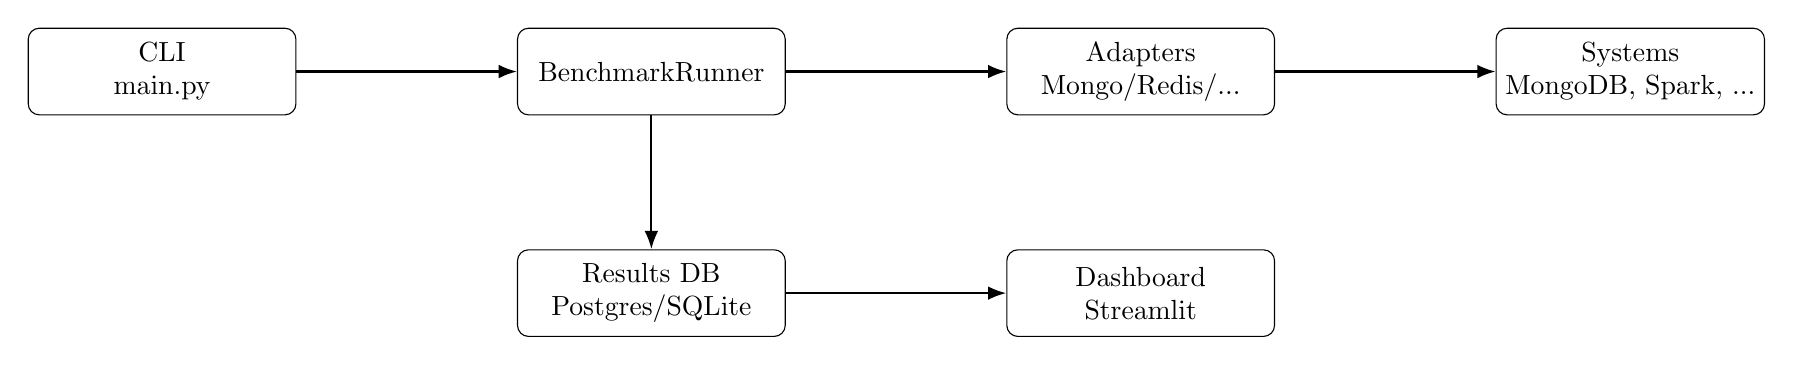
\begin{tikzpicture}[
  box/.style={draw, rounded corners, align=center, minimum width=3.4cm, minimum height=1.1cm},
  arrow/.style={-Latex, thick}
]
\node[box] (cli) {CLI\\main.py};
\node[box, right=2.8cm of cli] (runner) {BenchmarkRunner};
\node[box, right=2.8cm of runner] (adapter) {Adapters\\Mongo/Redis/...};
\node[box, right=2.8cm of adapter] (systems) {Systems\\MongoDB, Spark, ...};
\node[box, below=1.7cm of runner] (storage) {Results DB\\Postgres/SQLite};
\node[box, below=1.7cm of adapter] (dashboard) {Dashboard\\Streamlit};

\draw[arrow] (cli) -- (runner);
\draw[arrow] (runner) -- (adapter);
\draw[arrow] (adapter) -- (systems);
\draw[arrow] (runner) -- (storage);
\draw[arrow] (storage) -- (dashboard);
\end{tikzpicture}
\caption{PolyStoreBench overall architecture}
\end{figure}

\section{Adapter principle}
An adapter provides a unified interface for each system. The runner always calls the same set of
methods (load, insert, read, update, delete, query). This guarantees that each system is tested
with comparable operations, even if the internal implementation differs.

\chapter{Datasets and workloads}
\section{Supported formats}
The loader accepts two formats:
\begin{itemize}
  \item JSON (array or JSON Lines)
  \item CSV (with a header row)
\end{itemize}

\section{Schema-agnostic loading}
The loader does not assume any field names. It parses each row into a Python dictionary. If a JSON
array contains non-dict values, they are wrapped into a dictionary under the key \texttt{value} and
an internal index is added. There is no field casting such as \texttt{id} or \texttt{price}.

\section{Internal canonical schema (used by Hive and Cassandra)}
Systems that require a fixed table schema store each row as a generic payload:
\begin{longtable}{ll}
\toprule
Field & Description \\
\midrule
id & Auto-generated integer row id \\
payload & JSON string containing the original record \\
updated & Boolean flag used by the update operation \\
\bottomrule
\end{longtable}

\section{Example dataset generation (optional)}
The project includes a generator that creates a sales-like dataset. This is only an example; any
CSV or JSON dataset can be used.

\begin{lstlisting}[caption={Simplified example dataset generator}]
for i in range(n):
    record = {
        "id": i,
        "customer_name": fake.name(),
        "product": fake.word(),
        "category": random.choice(["tech", "books", "fashion", "food"]),
        "price": round(random.uniform(5, 1000), 2),
        "quantity": random.randint(1, 10),
        "timestamp": fake.iso8601()
    }
    data.append(record)
\end{lstlisting}

\section{Workloads}
Workloads are defined by:
\begin{itemize}
  \item Operation (insert, read, update, delete, query)
  \item Dataset size
  \item Concurrency level
  \item Number of repetitions
\end{itemize}
These definitions exist in YAML, but current execution is driven by BAT scripts and the CLI.

\chapter{Full execution flow (step by step)}
\section{Step 1 -- CLI launch}
A typical command looks like:
\begin{verbatim}
python main.py --system mongodb --operation insert --dataset data\any_dataset.json --size 10000 --scenario insert_test
\end{verbatim}

\section{Step 2 -- Adapter creation}
The CLI instantiates the adapter for the selected system (MongoDBAdapter, RedisAdapter, etc.).

\section{Step 3 -- Runner creation}
The runner receives the adapter and system name. It orchestrates timing and metrics.

\section{Step 4 -- Dataset loading}
The runner calls:\\
\texttt{adapter.load\_data(dataset\_path)}

This reads the file and keeps a list of records in memory. Each record is a dictionary; no
fixed schema is required.

\section{Step 5 -- Measurement and execution}
The runner starts a timer, runs the operation, and measures latency. For concurrent reads, it
creates multiple threads.

\begin{figure}[H]
\centering
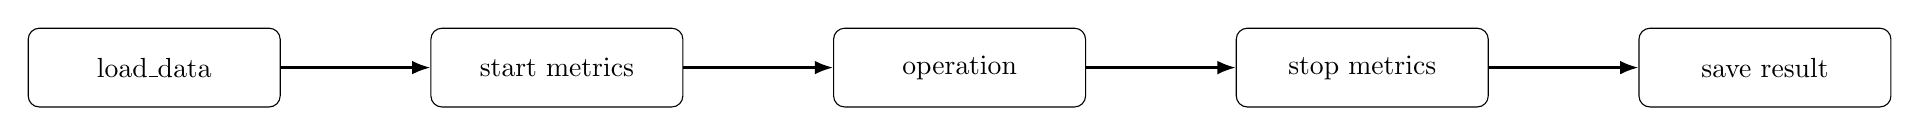
\begin{tikzpicture}[
  box/.style={draw, rounded corners, align=center, minimum width=3.2cm, minimum height=1cm},
  arrow/.style={-Latex, thick}
]
\node[box] (load) {load\_data};
\node[box, right=1.9cm of load] (start) {start metrics};
\node[box, right=1.9cm of start] (op) {operation};
\node[box, right=1.9cm of op] (stop) {stop metrics};
\node[box, right=1.9cm of stop] (save) {save result};

\draw[arrow] (load) -- (start);
\draw[arrow] (start) -- (op);
\draw[arrow] (op) -- (stop);
\draw[arrow] (stop) -- (save);
\end{tikzpicture}
\caption{Minimal benchmark pipeline}
\end{figure}

\section{Step 6 -- Metrics computation}
The runner computes:
\begin{itemize}
  \item Average latency in ms
  \item Min and max latency
  \item Total execution time in seconds
  \item Throughput in operations per second
\end{itemize}
Throughput formula:
\[ \text{throughput} = \frac{\text{op\_count}}{\text{execution\_time}} \]

\section{Step 7 -- Resource collection}
After the operation ends, the collector reads CPU, RAM, and disk usage via \texttt{psutil}. This is
a snapshot of the host system at benchmark time.

\section{Step 8 -- Result storage}
Results are stored in a database. PostgreSQL is used when available, otherwise SQLite.

\section{Step 9 -- Visualization}
The Streamlit dashboard reads result rows and displays comparative charts.

\chapter{Benchmark runner}
\section{Role}
The runner enforces consistent measurement across all systems and operations.

\section{Core pseudo-code}
\begin{lstlisting}[caption={Runner pseudo-code}]
adapter.load_data(path)
start_metrics()
start_timer()

if operation == "read" and concurrency > 1:
    run_concurrent_reads()
else:
    adapter.operation()

stop_timer()
stop_metrics()
compute_stats()
save_result()
\end{lstlisting}

\section{Concurrent reads}
The runner supports multi-threaded reads:
\begin{itemize}
  \item N threads are created (concurrency level)
  \item each thread performs 20 reads
  \item throughput and latencies are computed across all reads
\end{itemize}

\chapter{Adapter design}
\section{Common interface}
Each adapter implements the same methods:
\begin{itemize}
  \item load\_data()
  \item insert\_data()
  \item read\_data()
  \item update\_data()
  \item delete\_data()
  \item run\_query() (optional)
\end{itemize}

\begin{figure}[H]
\centering
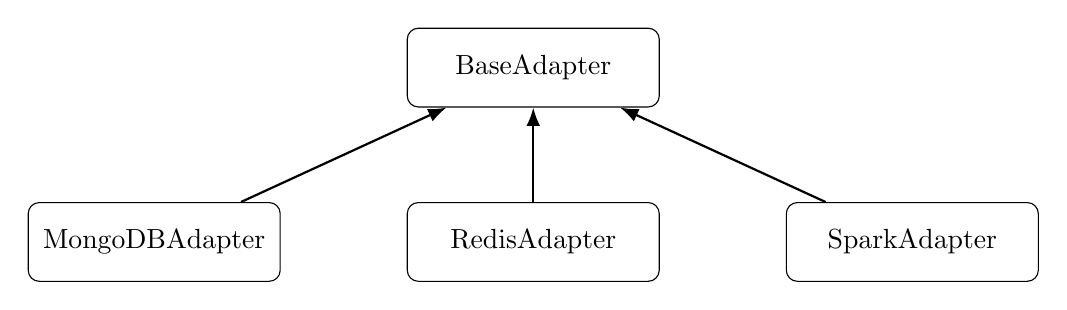
\begin{tikzpicture}[
  box/.style={draw, rounded corners, align=center, minimum width=3.2cm, minimum height=1cm},
  arrow/.style={-Latex, thick}
]
\node[box] (base) {BaseAdapter};
\node[box, below left=1.2cm and 1.6cm of base] (mongo) {MongoDBAdapter};
\node[box, below=1.2cm of base] (redis) {RedisAdapter};
\node[box, below right=1.2cm and 1.6cm of base] (spark) {SparkAdapter};

\draw[arrow] (mongo) -- (base);
\draw[arrow] (redis) -- (base);
\draw[arrow] (spark) -- (base);
\end{tikzpicture}
\caption{Shared adapter interface}
\end{figure}

\chapter{System details}
\section{MongoDB}
\begin{itemize}
  \item insert: clears the collection and inserts all records with a \texttt{\_psb\_id}
  \item read: reads 100 documents
  \item update: sets a generic \texttt{\_psb\_updated} flag
  \item delete: removes all documents
  \item query: returns a count of documents
\end{itemize}

\section{Redis}
\begin{itemize}
  \item insert: \texttt{flushdb} and store each record as JSON with key \texttt{record:<index>}
  \item read: scans up to 100 keys
  \item update: sets a generic \texttt{\_psb\_updated} flag in each JSON
  \item delete: \texttt{flushdb}
  \item query: counts all keys
\end{itemize}

\section{Cassandra}
\begin{itemize}
  \item creates a generic table with \texttt{id}, \texttt{payload}, \texttt{updated}
  \item insert: stores each record as a JSON string in \texttt{payload}
  \item read: SELECT LIMIT 100
  \item update: sets \texttt{updated=true} for all rows
  \item delete: TRUNCATE
  \item query: SELECT COUNT(*)
\end{itemize}

\section{Spark}
\begin{itemize}
  \item insert: loads file, caches, and materializes with count()
  \item read: collects 100 rows
  \item update: adds a generic \texttt{\_psb\_updated} column
  \item delete: unpersist cached DataFrame
  \item query: GROUP BY \texttt{category} if available, otherwise COUNT
\end{itemize}

\section{Hadoop (HDFS)}
\begin{itemize}
  \item insert: docker cp + hdfs dfs -put
  \item read: hdfs dfs -cat, read first KB
  \item update: re-upload (HDFS is immutable)
  \item delete: hdfs dfs -rm -r
  \item query: hdfs dfs -count
\end{itemize}

\section{Hive}
\begin{itemize}
  \item insert: converts dataset to a generic CSV (id, payload, updated) and LOAD DATA
  \item read: SELECT LIMIT 100
  \item update: INSERT OVERWRITE with updated=true
  \item delete: TRUNCATE TABLE
  \item query: SELECT COUNT(*)
\end{itemize}

\chapter{Metrics}
\section{Latency}
Latency measures the time of a single operation. For reads, the average latency is computed across
100 reads (or across all concurrent reads).

\section{Total time}
Total time is measured between the start and end of the operation.

\section{Throughput}
Throughput is the number of operations divided by total time.

\section{Resources}
CPU, RAM, and disk are collected via \texttt{psutil}. These are host-level percentages.

\chapter{Result storage}
\section{Logical schema}
Results are saved with the following fields:
\begin{itemize}
  \item system\_name, scenario\_name, operation, dataset\_size
  \item execution\_time\_sec, latency\_avg\_ms, latency\_min\_ms, latency\_max\_ms
  \item throughput\_ops\_sec
  \item cpu\_percent, memory\_percent, disk\_percent
  \item concurrency\_level, run\_number, created\_at
\end{itemize}

\begin{figure}[H]
\centering
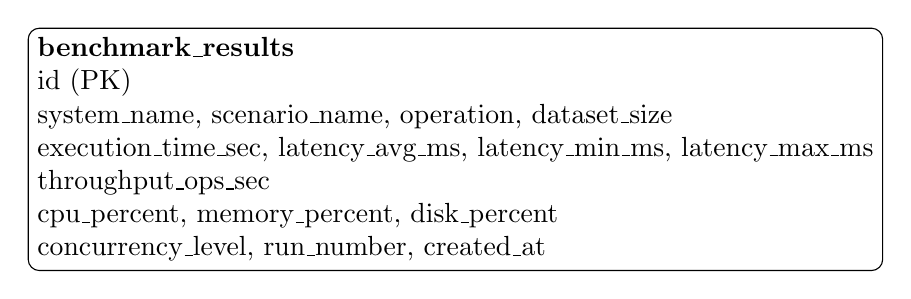
\begin{tikzpicture}[
  box/.style={draw, rounded corners, align=left, minimum width=9cm, minimum height=2.6cm},
  arrow/.style={-Latex, thick}
]
\node[box] (table) {
\textbf{benchmark\_results}\\
 id (PK)\\
 system\_name, scenario\_name, operation, dataset\_size\\
 execution\_time\_sec, latency\_avg\_ms, latency\_min\_ms, latency\_max\_ms\\
 throughput\_ops\_sec\\
 cpu\_percent, memory\_percent, disk\_percent\\
 concurrency\_level, run\_number, created\_at
};
\end{tikzpicture}
\caption{Logical schema of stored results}
\end{figure}

\section{PostgreSQL and SQLite}
PostgreSQL is used when available. If the connection fails, a local SQLite database is created
to allow offline usage.

\chapter{Dashboard}
\section{Role}
The dashboard is a Streamlit app that:
\begin{itemize}
  \item loads results from the database
  \item filters by system, operation, and size
  \item displays comparative charts
  \item accepts any dataset schema during upload
\end{itemize}

\begin{figure}[H]
\centering
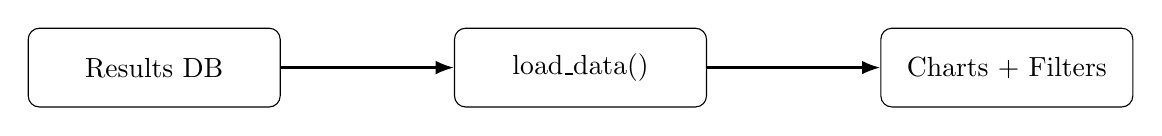
\begin{tikzpicture}[
  box/.style={draw, rounded corners, align=center, minimum width=3.2cm, minimum height=1cm},
  arrow/.style={-Latex, thick}
]
\node[box] (db) {Results DB};
\node[box, right=2.2cm of db] (load) {load\_data()};
\node[box, right=2.2cm of load] (ui) {Charts + Filters};
\draw[arrow] (db) -- (load);
\draw[arrow] (load) -- (ui);
\end{tikzpicture}
\caption{Dashboard flow}
\end{figure}

\chapter{Deployment and execution}
\section{Docker services}
Core services are defined in docker-compose:
\begin{itemize}
  \item MongoDB
  \item Redis
  \item PostgreSQL
  \item Cassandra
  \item Hadoop Namenode/Datanode
  \item Hive Server + Metastore
\end{itemize}

\section{Execution scripts}
BAT scripts run benchmark suites per system. For example:
\begin{itemize}
  \item run\_all.bat: full suite
  \item run\_spark.bat: Spark only
  \item run\_hive.bat: Hive only
\end{itemize}

\chapter{Beginner workflow}
\section{1. Start services}
Run Docker Compose to start the required services.

\section{2. Initialize the results database}
Run the init script to create the results table if needed.

\section{3. Run benchmarks}
Use a BAT script or the CLI directly.

\section{4. Open the dashboard}
Launch Streamlit and inspect the charts.

\chapter{Limitations and improvements}
\begin{itemize}
  \item Queries are generic counts, not domain-specific analytics
  \item Hive and Cassandra drop and recreate the benchmark table for schema safety
  \item Resource metrics are host-level, not per container
  \item No multi-node scaling tests
  \item YAML workloads are not executed by the runner yet
\end{itemize}

\chapter{Conclusion}
PolyStoreBench provides a solid base for comparing heterogeneous storage systems with a single,
consistent benchmark flow. Its main strength is the unified execution pipeline and automatic
result collection and visualization. With incremental enhancements, it can serve both academic
and industrial evaluation scenarios.

\appendix
\chapter{Useful code excerpts}
\section{Adapter interface}
\begin{lstlisting}[caption={Base adapter interface}]
class BaseAdapter(ABC):
    def load_data(self, dataset_path):
        pass
    def insert_data(self):
        pass
    def read_data(self):
        pass
    def update_data(self):
        pass
    def delete_data(self):
        pass
    def run_query(self):
        return None
\end{lstlisting}

\section{Metrics collection}
\begin{lstlisting}[caption={CPU/RAM/Disk collection}]
return {
    "cpu_percent": psutil.cpu_percent(interval=0.5),
    "memory_percent": psutil.virtual_memory().percent,
    "disk_percent": psutil.disk_usage(path).percent
}
\end{lstlisting}

\section{Example command}
\begin{verbatim}
python main.py --system redis --operation read --dataset data\any_dataset.json --size 10000 --scenario read_any
\end{verbatim}

\end{document}
